\documentclass[xcolor=table,dvipsnames,svgnames,aspectratio=169,fontset=ubuntu]{ctexbeamer}
% 可以通过 fontset=macnew / fontset=ubuntu / fontset=windows 选项切换字体集
\usepackage{tikz}
\usepackage[normalem]{ulem}
\usetikzlibrary{arrows}
\usepackage{amsmath}
\usepackage{mflogo}
\usepackage{graphicx}
\usepackage{ccicons}
\usepackage{hologo}
\usepackage{colortbl}
\usepackage{shapepar}
\usepackage{hyperxmp}
\usepackage{booktabs}
\usepackage{qrcode}
\usepackage{listings}
\usepackage{tipa}
\usepackage{multicol}
\usepackage{datetime2}
\usepackage{fontawesome5}
\usepackage{hyperref}
\usepackage{enumitem}
\usepackage{bm}
\usepackage[backend=biber,style=gb7714-2015]{biblatex}
\addbibresource{thesis.bib}
\graphicspath{{figures/}}
\hypersetup{
  pdfsubject = {上海交通大学图书馆专题培训讲座},
  pdfauthor = {Alexara Wu},
  pdfcopyright = {Licensed under CC-BY-SA 4.0. Some rights reserved.},
  pdflicenseurl = {http://creativecommons.org/licenses/by-sa/4.0/},
  unicode = true,
  psdextra = true,
  pdfdisplaydoctitle = true
}

\DeclareOptionBeamer{en}

\pdfstringdefDisableCommands{
  \let\\\relax
  \let\quad\relax
  \let\hspace\@gobble
}
\renewcommand{\TeX}{\hologo{TeX}}
\renewcommand{\LaTeX}{\hologo{LaTeX}}
\newcommand{\BibTeX}{\hologo{BibTeX}}
\newcommand{\XeTeX}{\hologo{XeTeX}}
\newcommand{\pdfTeX}{\hologo{pdfTeX}}
\newcommand{\LuaTeX}{\hologo{LuaTeX}}
\newcommand{\MiKTeX}{\hologo{MiKTeX}}
\newcommand{\MacTeX}{Mac\hologo{TeX}}
\newcommand{\beamer}{\textsc{beamer}}
\newcommand{\XeLaTeX}{\hologo{Xe}\kern-.13em\LaTeX{}}
\newcommand{\pdfLaTeX}{pdf\LaTeX{}}
\newcommand{\LuaLaTeX}{Lua\LaTeX{}}
\def\TeXLive{\TeX{} Live}
\let\TL=\TeXLive
\newcommand{\SJTUThesis}{\textsc{SJTUThesis}}
\newcommand{\SJTUThesisVersion}{1.1.0}
\newcommand{\SJTUThesisDate}{2023/3/24}
\newcommand{\SJTUBeamer}{\textsc{SJTUBeamer}}
\newcommand{\SJTUBeamerVersion}{3.0.0}
\newcommand{\SJTUBeamerDate}{2022/11/22}
\newcommand\link[1]{\href{#1}{\faLink}}
\newcommand\pkg[1]{\texttt{#1}}
\def\cmd#1{\texttt{\color{structure}\footnotesize $\backslash$#1}}
\def\env#1{\texttt{\color{structure}\footnotesize #1}}
\def\cmdxmp#1#2#3{\small{\texttt{\color{structure}$\backslash$#1}\{#2\}
\hspace{1em}\\ $\Rightarrow$\hspace{1em} {#3}\par\vskip1em}}
\lstset{
  language=[LaTeX]TeX,
  basicstyle=\ttfamily\footnotesize,
  tabsize=2,
  keywordstyle=\bfseries\ttfamily\color{cprimary},
  commentstyle=\sl\ttfamily\color[RGB]{100,100,100},
  stringstyle=\ttfamily\color[RGB]{50,50,50},
  extendedchars=true,
  breaklines=true,
}

\usetheme[maxplus,blue,smoothbars]{sjtubeamer}
% 使用 maxplus/max/min 切换标题页样式
% 使用 red/blue 切换主色调
% 使用 light/dark 切换亮/暗色模式
% 使用外样式关键词以获得不同的边栏样式
%   miniframes infolines  sidebar
%   default    smoothbars split	 
%   shadow     tree       smoothtree
% 使用 topright/bottomright 切换徽标位置
% 使用逗号分隔列表以同时使用多种选项

\author{上海交通大学学生创新中心}
\date{\the\year \,.\the\month \,}
%\subject{LaTeX, 论文排版, SJTUThesis}
\title[流形上的Soblev不等式与嵌入]
{\textnormal{线性规划与整数规划}} 

\setbeamercolor{block title alerted}{use=structure,fg=white,bg=structure.fg!88!black}
\setbeamercolor{block body alerted}{parent=normal text,use=block title,bg=block title.bg!10!white}


%=================================================================
%==================================================================

\begin{document}

\maketitle
%-----------------------------------------------------------------------
\section{数学规划}
\begin{frame}{什么是数学规划}
  数学规划,也称数学优化,是数学中的一个分支
  \vskip 12pt
  它主要研究:\underline{在给定的区域中可以最小化或最大化某一目标函数的最优解}。
  \vskip 12pt
  数学规划包括\underline{线性规划、整数规划}、非线性规划、动态规划、目标规划等等。
\end{frame}

\begin{frame}{数学规划的应用}
  \begin{columns}
    \column{0.5\textwidth}
    \begin{itemize}
      \item 1.吉尼斯世界纪录
      \vskip 15pt
      \item 2.总理的政府工作报告
      \vskip 15pt
      \item 3.公司领导的核心工作
      \vskip 15pt
      \item 4.如何使用好自己的钱
    \end{itemize}
    \column{0.5\textwidth}
    \begin{itemize}
      \item 5.树木的生长问题
      \vskip 15pt
      \item 6.群狼的捕猎计划
      \vskip 15pt
      \item 7.地铁车次的安排 
      \vskip 15pt
      \item 8.原子的内部结构
    \end{itemize}
  \end{columns}
  \vskip 30pt
  问题:你还能将想到哪些数学规划的应用?
\end{frame}

\section{线性规划}

\begin{frame}{线性规划的实例与定义}
  【例1】某机床厂生产甲、乙两种机床,每台销售后的利润分别为 4000 元与 3000 元。

  \vskip 5pt
  生产甲机床需用 A、B 机器加工,加工时间分别为每台 2 小时和 1 小时;
  
  \vskip 5pt
  生产乙机床需用 A、B、C 三种机器加工,加工时间为每台各1小时。
  
  \vskip 5pt
  若每天可用于加工的机器时数分别为 A 机器 10 小时、B 机器 8 小时和 C 机器 7 小时,问该厂应生产甲、乙机床各
几台,才能使总利润最大?
\end{frame}

\begin{frame}{线性规划的实例与定义}
  \begin{columns}
    \column{0.5\textwidth}

    (目标函数) $\max z=4 x_1+3 x_2$

    \vskip 15pt
    s.t. (约束条件) $\left\{\begin{array}{l}2 x_1+x_2 \leq 10 \\ x_1+x_2 \leq 8 \\ x_2 \leq 7 \\ x_1, x_2 \geq 0\end{array}\right.$

    \column{0.5\textwidth}
    设 $x_1$ 台甲机床, $x_2$ 台乙机床,

    变量 $x_1,x_2$ 称之为决策变量,
    \vskip 5pt
    (1)式被称为问题的目标函数
    \vskip 5pt
    (2)中的几个不等式是问题的约束条件,记为 s.t.(即 subject to)
    \vskip 5pt
    由于上面的目标函数及约束条件均为线性函数,故被称为线性规划问题
\end{columns}

\vskip 20pt
\begin{alertblock}{线性规划问题=目标函数+约束条件}
线性规划问题是在一组线性约束条件的限制下,求一线性目标函数的最大或最小值
\end{alertblock}
\end{frame}

\begin{frame}{尝试用画图的方法找到最大值}
  \begin{columns}
    \column{0.5\textwidth}

    (目标函数) $\max z=4 x_1+3 x_2$

    \vskip 15pt
    s.t. (约束条件) $\left\{\begin{array}{l}2 x_1+x_2 \leq 10 \\ x_1+x_2 \leq 8 \\ x_2 \leq 7 \\ x_1, x_2 \geq 0\end{array}\right.$

    \column{0.5\textwidth}
    提示:考虑$x_1,x_2$平面,将目标问题与约束条件转化为平面上的直线和区域
  \end{columns}
\end{frame}

\begin{frame}{尝试用画图的方法找到最大值}
  \begin{columns}
    \column{0.4\textwidth}

    $\max z=4 x_1+3 x_2$

    \vskip 15pt
    s.t. $\left\{\begin{array}{l}2 x_1+x_2 \leq 10 \\ x_1+x_2 \leq 8 \\ x_2 \leq 7 \\ x_1, x_2 \geq 0\end{array}\right.$
    \vskip 15pt
    最优解$x_1=2,x_2=6$
    
    最大利润$z_{max}=26$
    \column{0.4\textwidth}
    \begin{figure}
      \centering
      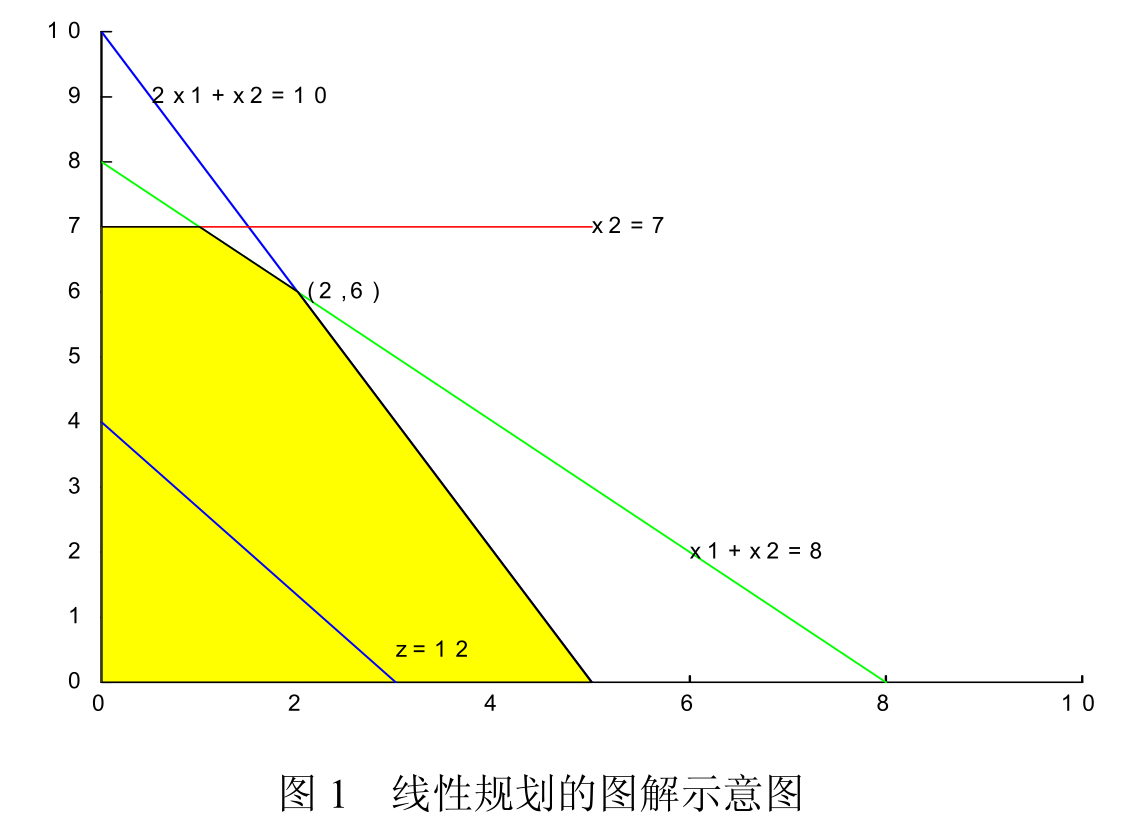
\includegraphics[width=1.2\textwidth]{绘图法.png}
    \end{figure}
  \end{columns}
\end{frame}

\begin{frame}{Matlab求解线性规划问题}
思考:为什么要用借助计算机求解线性规划问题?
\vskip 20pt
提示:问题的维数、约束条件的数量、可行域的复杂程度……
\end{frame}


\begin{frame}{线性规划的Matlab标准形式}
  线性规划的目标函数可以是求最大值,也可以是求最小值;
  
  约束条件的不等号可以是小于号,也可以是大于号;
  
  为了避免这种形式多样性带来的不便,Matlab 中规定线性
规划的标准形式为:

$$\begin{aligned} & \min c^T x \\ & \text { s.t. }\left\{\begin{array}{l}A x \leq b \\ A e q \cdot x=b e q \\ l b \leq x \leq u b\end{array}\right.\end{aligned}$$

\vskip 10pt
$c$ 和 $x$ 为 $n$ 维列向量, $A$ 、 $Aeq$ 为适当维数的矩阵, $b$ 、 $beq$ 为适当维数的列向量

\end{frame}

\begin{frame}{Matlab求解线性规划问题}
  \begin{columns}
    \column{0.4\textwidth}
    【例2】Step1:转化为标准形式
    \vskip 10pt
    $\begin{aligned} & \max z=2 x_1+3 x_2-5 x_3 \\ \text { s.t. } & x_1+x_2+x_3=7 \\ & 2 x_1-5 x_2+x_3 \geq 10 \\ & x_1+3 x_2+x_3 \leq 12 \\ & x_1, x_2, x_3 \geq 0\end{aligned}$    
    \column{0.6\textwidth}
    $\begin{aligned}  \min -z&=-2 x_1-3 x_2+5 x_3\\& =(-2,-3,5)(x_1,x_2,x_3) \\
      x_1+x_2+x_3&=(1,1,1)(x_1,x_2,x_3)=7 \\
      -2 x_1+5 x_2-x_3 &=(-2,5,-1)(x_1,x_2,x_3)\leq 10 \\
      x_1+3 x_2+x_3 &=(1,3,1)(x_1,x_2,x_3)\leq 12 \\
      x_1, x_2, x_3 &=(x_1,x_2,x_3)\geq 0\\
      \end{aligned}$    
  \end{columns}
\end{frame}

\begin{frame}{Matlab求解线性规划问题}
  \begin{columns}
    \column{0.4\textwidth}
    【例2】Step2:写出对应的参量
    \vskip 10pt
    $\begin{aligned}  &c=[-2;-3;5];\\
      &a=[-2,5,-1;1,3,1];\\ 
      &b=[-10;12];\\
      &aeq=[1,1,1];\\
      &beq=7;\\
    \end{aligned}$   
    \column{0.6\textwidth}
    $\begin{aligned}  \min -z&=-2 x_1-3 x_2+5 x_3\\& =(-2,-3,5)(x_1,x_2,x_3) \\
      x_1+x_2+x_3&=(1,1,1)(x_1,x_2,x_3)=7 \\
      -2 x_1+5 x_2-x_3 &=(-2,5,-1)(x_1,x_2,x_3)\leq -10 \\
      x_1+3 x_2+x_3 &=(1,3,1)(x_1,x_2,x_3)\leq 12 \\
      x_1, x_2, x_3 &=(x_1,x_2,x_3)\geq 0\\
      \end{aligned}$    
  \end{columns}
\end{frame}

\begin{frame}{Matlab求解线性规划问题}
  \begin{columns}
    \column{0.5\textwidth}
    【例2】Step3:写出相应Matlab代码
    \vskip 10pt
    $\begin{aligned}  &c=[-2;-3;5];\\
      &a=[-2,5,-1;1,3,1];\\ 
      &b=[-10;12];\\
      &aeq=[1,1,1];\\
      &beq=7;\\
    \end{aligned}$   
    \column{0.5\textwidth}
    \begin{alertblock}{例2 Matlab求解}
      c=[-2;-3;5];\\
      a=[-2,5,-1;1,3,1]; \\
      b=[-10;12];\\
      aeq=[1,1,1];\\
      beq=7;\\
      x=linprog(c,a,b,aeq,beq,zeros(3,1))\\
      value=(-c)'*x
    \end{alertblock}
  \end{columns}
\end{frame}

\begin{frame}{Matlab求解线性规划问题}
  \begin{columns}
    \column{0.5\textwidth}
    【例3】求解线性规划问题
    \vskip 10pt
    $\begin{aligned} & \min z=2 x_1+3 x_2+x_3 \\ s.t. & \left\{\begin{array}{l}x_1+4 x_2+2 x_3 \geq 8 \\ 3 x_1+2 x_2 \geq 6 \\ x_1, x_2, x_3 \geq 0\end{array}\right.\end{aligned}$ 
    \column{0.5\textwidth}
    \begin{alertblock}{例3 Matlab求解}
      c=[2;3;1];\\
      a=[1,4,2;3,2,0];\\
      b=[8;6];\\
      \text{[x,y]=linprog(c,-a,-b,[],[],zeros(3,1))}\\
      value=c'*x
    \end{alertblock}  
  \end{columns}
\end{frame}

\begin{frame}{线性规划问题的建模与求解}
  【例4】某化工厂根据一项合同要求为用户生产一种用甲、乙两种原料混合配制而成的特种产品。已知甲、乙两种原料都含有A、B、C三种化学成分, 两种原料分别所含三种化学成分的百分比含量, 以及按合同规定的产品中三种化学成分的最低含量如下表所示:
  
  \vskip 10pt
  \begin{tabular}{|c|c|c|c|}
    \hline 化学成分 & 甲(\%) & 乙(\%) & 产品最低含量(\%) \\
    \hline B & 12 & 3 & 2 \\
    \hline C & 2 & 3 & 5 \\
    \hline
  \end{tabular}
  
  \vskip 10pt

  已知甲、乙两种原料的成本分别是每公斤3元和2元, 厂方希望总成本达到最小, 问如何配置该产品?
\end{frame}

\begin{frame}{线性规划问题的建模与求解}
  定义 $x_1, x_2$ 分别为每公斤产品中甲, 乙两种原料的数量,
  
  \vskip 10pt
  目标: 使总成本最小化 $\qquad\qquad\qquad\qquad\qquad\quad \min z=3 x_1+2 x_2$

  \vskip 10pt
  约束: 配料平衡条件, $\qquad\qquad\qquad\qquad\qquad\qquad\quad x_1+x_2=1$
  
  \vskip 10pt
  产品中 A、B、C三种化学成分的最低含量
  $ \qquad \begin{array}{r}
  12 x_1+3 x_2 \geq 4 \\
  2 x_1+3 x_2 \geq 2 \\
  3 x_1+15 x_2 \geq 5 
  \end{array}  $

  \vskip 10pt
  非负性条件  $\qquad\qquad\qquad\qquad\qquad\qquad\qquad\qquad x_1 \geq 0, x_2 \geq 0$
\end{frame}

\begin{frame}{线性规划问题的建模与求解}
  \begin{columns}
    \column{0.6\textwidth}
    \begin{alertblock}{例4 Matlab求解}
      c=[3;2];\\
      a=[12,3;2,3;3,15];\\
      b=[4;2;5];\\
      aeq=[1,1];\\
      beq=1;\\
      x=linprog(c,-a,-b,aeq,beq,zeros(2,1))\\
      value=c'*x
    \end{alertblock}
    \column{0.4\textwidth}
    $x_1=0.1111$
    \vskip 15pt
    $x_2=0.8889$
    \vskip 15pt
    $z_{min}=2.1111$
    \end{columns}
\end{frame}


\section{整数规划}

\begin{frame}{整数规划的定义}
  规划中的变量(部分或全部)限制为整数时,称为整数规划。

  \vskip 12pt

  若在线性规划模型中,变量限制为整数,则称为整数线性规划。

  \vskip 12pt

  目前还没有一种方法能有效地求解一切整数规划。
\end{frame}

\begin{frame}{整数规划的实例-低维数}
  \begin{columns}
    \column{0.4\textwidth}

    【例1】
    \vskip 10pt
    $\max z=4 x_1+3 x_2$

    \vskip 15pt
    s.t. $\left\{\begin{array}{l}2 x_1+x_2 \leq 10 \\ x_1+x_2 \leq 8 \\ x_2 \leq 7 \\ x_1, x_2 \geq 0\end{array}\right.$
    \vskip 15pt
    最优解$x_1=2,x_2=6$
    
    最大利润$z_{max}=26$
    \column{0.4\textwidth}
    \begin{figure}
      \centering
      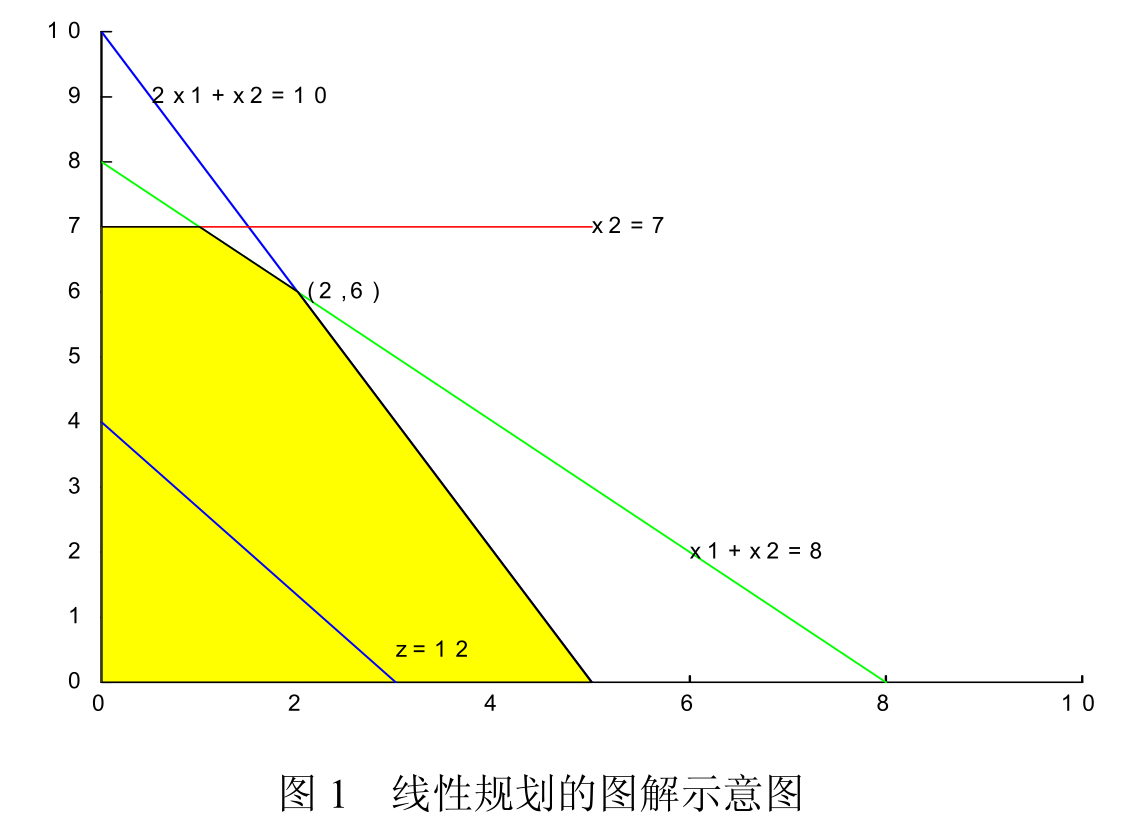
\includegraphics[width=1.2\textwidth]{绘图法.png}
    \end{figure}
  \end{columns}
\end{frame}

\begin{frame}{整数规划的实例-高维数}
  【例5】
$$\begin{aligned} & \operatorname{Max} z=x_1^2+x_2^2+3 x_3^2+4 x_4^2+2 x_5^2-8 x_1-2 x_2-3 x_3-x_4-2 x_5 \\ s.t.& \left\{\begin{array}{l}0 \leq x_i \leq 99 \quad(i=1, \cdots, 5) \\ x_1+x_2+x_3+x_4+x_5 \leq 400 \\ x_1+2 x_2+2 x_3+x_4+6 x_5 \leq 800 \\ 2 x_1+x_2+6 x_3 \leq 200 \\ x_3+x_4+5 x_5 \leq 200\end{array}\right.\end{aligned}$$
\end{frame}

\begin{frame}{整数规划的实例-高维数}
  $$\begin{aligned} & \operatorname{Max} z=x_1^2+x_2^2+3 x_3^2+4 x_4^2+2 x_5^2-8 x_1-2 x_2-3 x_3-x_4-2 x_5 \\ s.t.& \left\{\begin{array}{l}0 \leq x_i \leq 99 \quad(i=1, \cdots, 5) \\ x_1+x_2+x_3+x_4+x_5 \leq 400 \\ x_1+2 x_2+2 x_3+x_4+6 x_5 \leq 800 \\ 2 x_1+x_2+6 x_3 \leq 200 \\ x_3+x_4+5 x_5 \leq 200\end{array}\right.\end{aligned}$$

  \vskip 15pt
  如果用显枚举法试探,共需计算$(100)^5=10^{10}$个点,其计算量非常之大。
  
  \vskip 15pt
  然而蒙特卡洛法指出:随机计算$(10)^6$个点,便可找到满意解,为什么?
\end{frame}

\begin{frame}{整数规划的实例-高维数}
  \begin{columns}
    \column{0.5\textwidth}
    假设目标函数落在高值区的概率为 0.01
    
    \vskip 10pt
    则当计算$10^6$个点后,有任一个点能落在高值区的概率为:

    \vskip 10pt
    $1-0.99^{1000000} \approx 0.99 \cdots 99(100 \text { 多位) }$

    \column{0.55\textwidth}
    假设目标函数落在高值区的概率为 0.00001 
        
    \vskip 10pt
    则当计算$10^6$个点后,有任一个点能落在高值区的概率为:
  
    \vskip 10pt
    $1-0.99999^{1000000} \approx 0.999954602 $
  \end{columns}

  \vskip 30pt
  蒙特卡洛法不一定能找到精确解,但是可以找到一个“相对令人满意”的解。
\end{frame}

\begin{frame}{蒙特卡洛法的背景}
  \begin{columns}
    \column{0.6\textwidth}
  蒙特卡洛法作为一种计算方法,是由美国数学家乌拉姆(Ulam,S.M.)与美籍匈牙利数学家冯·诺伊曼(von Neumann,J.)在20世纪40年代中叶,为研制核武器的需要而首先提出来的。

  \vskip 15pt
  虽然利用蒙特卡罗方法估计的计算结果与精确值之间有误差,但是可以通过增加样本量或者改进抽样方法等方法降低计算误差,提高计算精度。
  \column{0.4\textwidth}
  \begin{figure}
    \centering
    
\includegraphics[width=0.6\textwidth]{abhm.jpeg}
  \end{figure}
\end{columns}
\end{frame}

\begin{frame}{蒙特卡洛法的应用}
\begin{columns}
  \column{0.5\textwidth}
  \begin{figure}
    \centering
    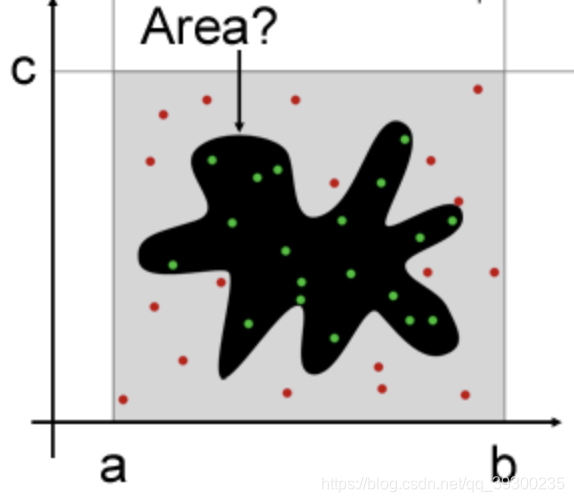
\includegraphics[width=0.8\textwidth]{mc求面积.png}
  \end{figure}
  \column{0.5\textwidth}
  估计不规则图形的面积:

  \vskip 10pt
  $$\begin{aligned}A_{\text {shape }} &\approx \frac{N_{\text {hits }}}{N_{\text {total }}} \times A\\&~\\ A&=a b \times a c\\\end{aligned}$$.
\end{columns}
\end{frame}

\begin{frame}{蒙特卡洛法求解整数规划问题}
  首先定义目标函数 $f$ 和约束向量函数 $g$,
  \begin{alertblock}{例5 Matlab求解}
    function [f,g]=mengte(x);\\
    f=x(1)\^{}2+x(2)\^{}2+3*x(3)\^{}2+4*x(4)\^{}2+2*x(5)\^{}2-8*x(1)-2*x(2)-3*x(3)-x(4)-2*x(5);\\
    g=[sum(x)-400;\\
    x(1)+2*x(2)+2*x(3)+x(4)+6*x(5)-800;\\
    2*x(1)+x(2)+6*x(3)-200;\\
    x(3)+x(4)+5*x(5)-200];\\
  \end{alertblock}
\end{frame}

\begin{frame}{蒙特卡洛法求解整数规划问题}
  然后求例5的解
  \begin{columns}
    \column{0.5\textwidth}  
    \begin{alertblock}{例5 Matlab求解}
      % 初始化随机数生成器,确保每次运行结果相同
      rand('state', sum(clock));
  
      % 初始化最优目标函数值和最优解
      p0 = 0;
      x0 = [];
  
      % 计时开始
      tic;\\
      % 循环生成随机解
      for i = 1:10\^{}6\\
      % 生成随机解
      x = 99 * rand(5, 1);\\
      % 取整和向上取整
      x1 = floor(x);\\
      x2 = ceil(x);
    \end{alertblock}
    \column{0.5\textwidth}
    \begin{alertblock}{例5 Matlab求解}
      % 计算当前解的目标函数和约束条件
      [f, g] = mente(x1);\\
      % 检查是否满足所有约束条件
      if sum(g <= 0) == 4
          % 检查是否是当前最优解
          if p0 <= f
              x0 = x1;
              p0 = f;
          end
      end

      % 对向上取整的解也进行同样的检查
      [f, g] = mente(x2);\\
      if sum(g <= 0) == 4
          if p0 <= f
              x0 = x2;
              p0 = f;
          end
      end\\
      end
    \end{alertblock}

  \end{columns}

\end{frame}

\begin{frame}{蒙特卡洛法求解整数规划问题}
  【例6】
  $$\begin{aligned} & \operatorname{Max} z=3x_1^2+x_2^2+3 x_3^2+2 x_4^2+4 x_5^2-8 x_1-4 x_2-16 x_3-5x_4-3 x_5 \\ s.t.& \left\{\begin{array}{l}0 \leq x_i \leq 99 \quad(i=1, \cdots, 5) \\ x_1+x_2+x_3+x_4+x_5 \leq 400 \\ x_1^2+2 x_2^2+2 x_3^2+x_4^2+6 x_5^2 \leq 800 \\ 2 x_1+x_2+6 x_3 \leq 200 \\ x_3^2+x_4^2+5 x_5^2 \leq 200\end{array}\right.\end{aligned}$$ 
\end{frame}

\begin{frame}{蒙特卡洛法求解整数规划问题}
  【例7】某铁器加工厂要制作 100 套钢架, 每套要用长为 2.9 米, 2.1 米和 1.5 米的圆钢各一根。已知原料长为 7.4 米, 问应如何下料, 可使材料最省?
\end{frame}

\begin{frame}{蒙特卡洛法求解整数规划问题}
  在长度确定的原料上截取三种不同规格的圆钢, 可以归纳出8种不同的下料方案:
  
  \vskip 15pt
  \begin{tabular}{|c|c|c|c|c|c|c|c|c|}
  \hline 圆钢 (米) & I & II & III & IV & V & VI & VII & VII \\
  \hline 2.9 & 1 & 2 & 0 & 1 & 0 & 1 & 0 & 0 \\
  \hline 2.1 & 0 & 0 & 2 & 2 & 1 & 1 & 3 & 0 \\
  \hline 1.5 & 3 & 1 & 2 & 0 & 3 & 1 & 0 & 4 \\
  \hline 料头 (米) & 0 & 0.1 & 0.2 & 0.3 & 0.8 & 0.9 & 1.1 & 1.4 \\
  \hline
  \end{tabular}
  
  \vskip 15pt
  问题归纳为:如何混合使用这 8 种不同的下料方案, 来制造1000套钢架, 且要使剩余的余料总长为最短。

\end{frame}

\begin{frame}{蒙特卡洛法求解整数规划问题}
  设 $x_j$ 表示用第 $j$ 种下料方案下料的原料根数, $j=1,2 \ldots, 8$
  
  \vskip 5pt
  目标: 使余料总长度最小化
  $$
  \min z=0 x_1+0.1 x_2+0.2 x_3+0.3 x_4+0.8 x_5+0.9 x_6+1.1 x_7+1.4 x_8
  $$
  
  约束: 三种规格圆钢根数
  $$
  \begin{aligned}
  x_1+2 x_2+x_4+x_6 & =100 \\
  2 x_3+2 x_4+x_5+x_6+3 x_7 & =100 \\
  3 x_1+x_2+2 x_3+3 x_5+x_6+4 x_8 & =100
  \end{aligned}
  $$
  
  非负取整条件
  $x_j \geq 0 (j=1,2 \ldots 8)$ 且取整数
\end{frame}







\makebottom


\end{document}
